\documentclass{beamer}

\usepackage[T1]{fontenc}
\usepackage[utf8]{inputenc}
\usepackage{unicode}
\usepackage[american]{babel}
\usepackage{amsmath,amssymb,amsthm}
\usepackage{tikz,pgflibraryarrows,pgflibraryplotmarks,pgflibrarysnakes,pgflibraryshapes}
\usepackage{tikzsymbols}
\usepackage[backend=biber,citestyle=authoryear-comp,bibstyle=beamer,doi=false,isbn=false,url=false,maxnames=10]{biblatex}
\usepackage[nosfdefault]{comicneue}
\usepackage[normalem]{ulem}
\bibliography{defeo}

\mode<presentation>{%
  \usetheme{Boadilla}
}
\beamertemplatenavigationsymbolsempty

\usepackage{sourcesanspro}
\usepackage[amssymb,amsfonts]{concmath}
\usefonttheme[onlymath]{serif}

\renewcommand{\emph}[1]{{\usebeamercolor[fg]{structure}#1}}

%\let\footcite\footnote

\newcommand{\C}{\mathbb{C}}
\newcommand{\R}{\mathbb{R}}
\newcommand{\Z}{\mathbb{Z}}
\newcommand{\N}{\mathbb{N}}
\newcommand{\Q}{\mathbb{Q}}
\newcommand{\F}{\mathbb{F}}
\renewcommand{\O}{\mathcal{O}}
\newcommand{\tildO}{\mathcal{\tilde{O}}}
\newcommand{\End}{\operatorname{End}}
\newcommand{\chr}{\operatorname{char}}
\newcommand{\Cl}{\operatorname{Cl}}
\renewcommand{\a}{{\mathfrak{a}}}
\renewcommand{\b}{{\mathfrak{b}}}
\newcommand{\cyc}[1]{{\langle #1 \rangle}}
\newcommand{\ord}{\operatorname{ord}}

\usetikzlibrary{matrix,decorations,decorations.text,calc,arrows,snakes,shapes,positioning}

\pgfkeys{/triangle/.code=\tikzset{x={(-0.5cm,-0.866cm)},y={(1cm,0cm)}}}
\pgfkeys{/lattice/.code n args={4}{\tikzset{cm={#1,#2,#3,#4,(0,0)}}}}

\newcommand{\axes}[4]{
  \clip (#1,#3) rectangle (#2,#4);
  \draw [thin, gray, -latex] (#1,0) -- (#2,0);% Draw x axis
  \draw [thin, gray, -latex] (0,#3) -- (0,#4);% Draw y axis
}

\newcommand{\lattice}[2]{
  \draw[style=help lines,dashed] (#1-1,#1-1) grid[step=1] (#2+1,#2+1);
  \foreach \x in {#1,...,#2}{
    \foreach \y in {#1,...,#2}{
      \node[draw,circle,inner sep=2pt,fill] at (\x,\y) {};
      % Places a dot at those points
    }
  }
}

\newcommand{\bl}[1]{\textcolor{blue}{#1}}
\newcommand{\rd}[1]{\textcolor{red}{#1}}
\newcommand{\gr}[1]{\textcolor{green}{#1}}

% This command defines a triangle of dots of given height
\newcommand{\dottriangle}[2][\i-\j]{%
  \foreach \i in {0,...,#2} {%
    \foreach \j in {0,...,\i} {%
      \draw(\i,\j) node{#1};%
    }%
  }}


\title[Isogeny graphs in cryptography]{
  Isogeny graphs in cryptography:\\
  the good, the bad and the ugly}
\author{Luca De Feo}
\date[Roma Tre, May 13, 2019]{May 13, 2019, Università di Roma 3, Roma}
\institute[UVSQ]{Université Paris Saclay -- UVSQ}

\begin{document}

\frame[plain]{
  \begin{tikzpicture}[remember picture,overlay]
    \node[at=(current page.center), opacity=0.5] {
      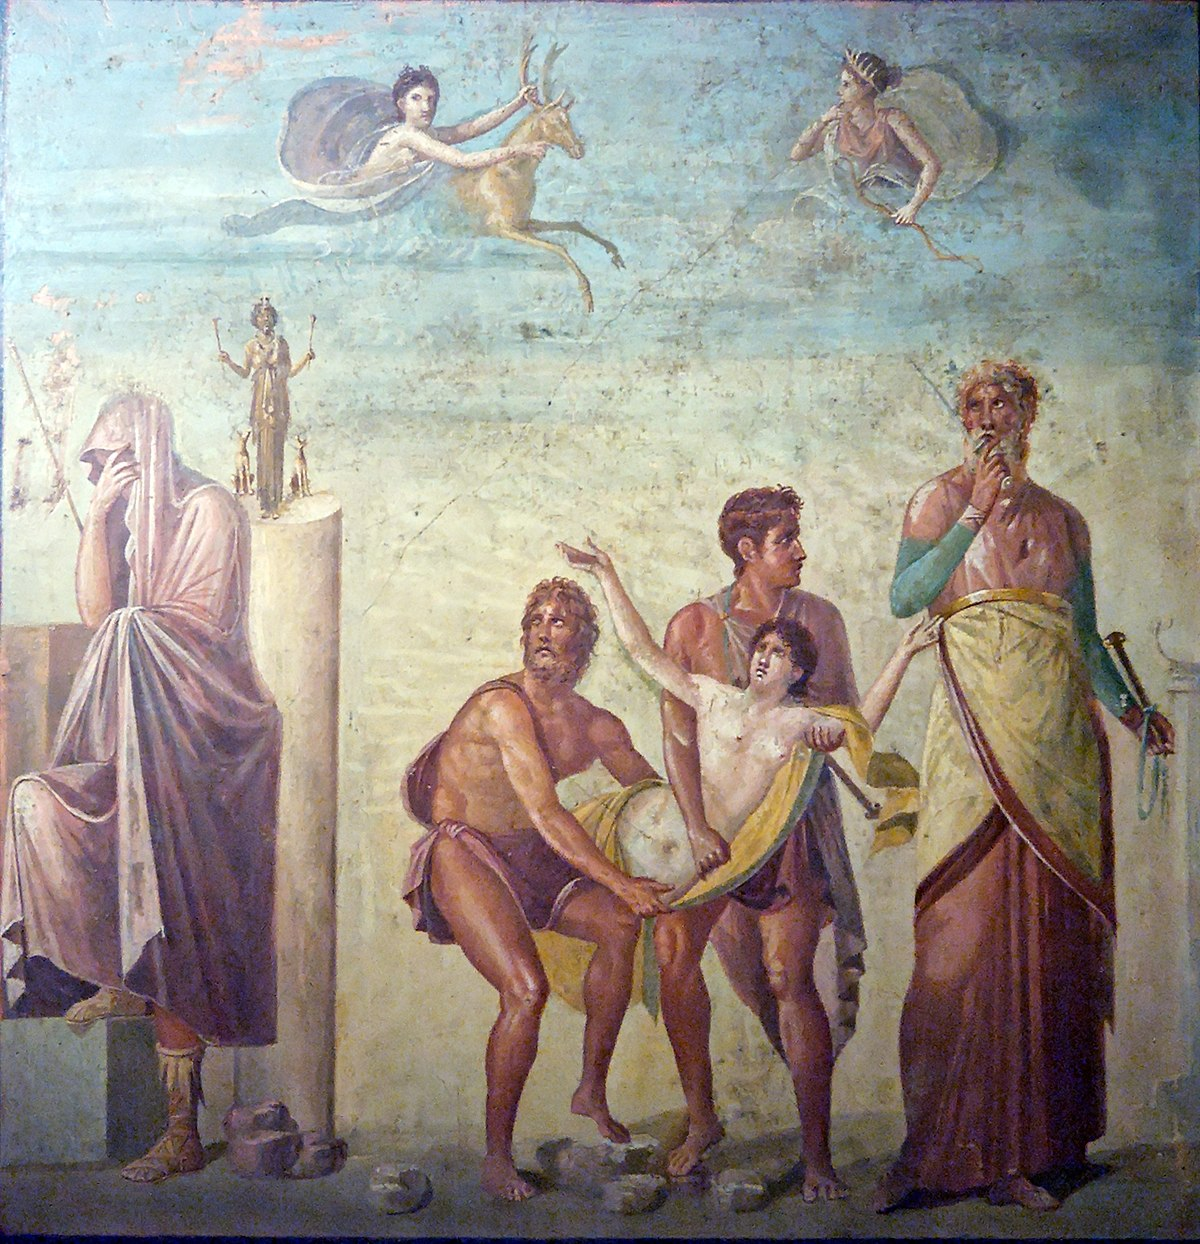
\includegraphics[width=1\paperwidth]{iphigenia.jpg}
    };
  \end{tikzpicture}
  \vspace{-1.1cm}
  \usebeamercolor[fg]{titlegraphic}
  {\bf \titlepage}
  \vspace{0.5cm}
  \begin{center}
    Slides online at~~~\textcolor{blue}{\href{https://defeo.lu/docet/}{https://defeo.lu/docet/}}
  \end{center}
}

%%

\begin{frame}{Elliptic curves}

  Let \emph{$E \;:\; y^2 = x^3 + ax + b$} be an elliptic curve\dots

  \begin{center}
    \begin{tikzpicture}[domain=-2.4566:4,samples=100]
      \newcount\rotate
      \animate<2-6>
      \animatevalue<2-6>{\rotate}{0}{90}
      \begin{scope}[rotate=-\the\rotate]
        \draw plot (\x,{0.5*sqrt(\x*\x*\x-4*\x+5)});
        \draw plot (\x,{-0.5*sqrt(\x*\x*\x-4*\x+5)});
      \end{scope}
      
      \begin{uncoverenv}<1>
        \begin{scope}[yscale=1/2]
          \draw[thin,gray,-latex] (0,-7) -- (0,7);
          \draw[thin,gray,-latex] (-3,0) -- (4,0);
          
          \draw (-3,1) -- (4,8/3+3);
          \begin{scope}[every node/.style={draw,circle,inner sep=1pt,fill},cm={1,2/3,0,0,(0,3)}]
            \node at (-2.287980,0) {};
            \node at (-0.535051,0) {};
            \node at (3.267475,0) {};
          \end{scope}
          \begin{scope}[every node/.style={yshift=0.3cm},cm={1,2/3,0,0,(0,3)}]
            \node at (-2.287980,0) {$P$};
            \node at (-0.535051,0) {$Q$};
            \node at (3.267475,0) {$R$};
          \end{scope}
          \draw[dashed] (3.267475,3.267475*2/3+3) -- (3.267475,-3.267475*2/3-3) 
          node[draw,circle,inner sep=1pt,fill] {}
          node[xshift=-0.1cm,anchor=east] {$P+Q$};
        \end{scope}
      \end{uncoverenv}
    \end{tikzpicture}
  \end{center}
\end{frame}

%%

\begin{frame}{Elliptic curves}
  \transdissolve
  \centering
  
\includegraphics[height=0.7\textheight]{ec-happy}

  \Large\bf I power 70\% of WWW traffic!
\end{frame}

%%

\begin{frame}{The Q Menace}
  \centering
  \includegraphics[height=0.7\textheight]{qc-ibm}
\end{frame}

%%

\begin{frame}{Post-quantum cryptographer?}
  \centering
  \includegraphics[height=0.7\textheight]{ec-broke}
\end{frame}

%%

\begin{frame}{Elliptic curves of the world, UNITE!}
  \centering
  \begin{tikzpicture}
    \foreach \x/\y in {0/-0.5,4/2,8/-1}{
      \node at (\x,\y) {\includegraphics[height=3cm]{ec-banderole}};
    }
    \foreach \x/\y in {1/3,4.5/-1,7/3}{
      \node at (\x,\y) {
\includegraphics[height=3.5cm]{ec-sign}};
    }
    \color{teal!70!blue}\itshape\bfseries\comicneue
    \node[rotate=-3] at (5.9,3.6) {\parbox{0pt}{QUOUSQUE\\QUANTUM?}};
    \node[rotate=-3] at (3.6,-0.4) {\parbox{0pt}{QUANTUM\\SUFFICIT!}};
  \end{tikzpicture}
\end{frame}

%%

\begin{frame}{And so, they found a way around the Q...}
  \centering
  \begin{tikzpicture}
    \comicneue\itshape
    \node at (0,0) {\includegraphics[height=2.5cm]{qc-ibm}};
    
    \node(E0) at (-5,0) {
\includegraphics[height=1cm]{ec-happy}};

    \uncover<2->{
      \node(EA) at (0,3.5) {
\includegraphics[height=1cm]{ec-happy}};
      \node(EB) at (0,-3.5) {
\includegraphics[height=1cm]{ec-happy}};
      \draw[->,decorate,decoration=snake] (E0) to (EA);
      \draw[->,decorate,decoration=snake] (E0) to (EB);
      \node[right=0.3cm of EA] {\bl{Public curve}};
      \node[right=0.3cm of EB] {\bl{Public curve}};
    }
    \uncover<3>{
      \node(ES) at (5,0) {
\includegraphics[height=1cm]{ec-happy}};
      \draw[->,decorate,decoration=snake] (EA) to (ES);
      \draw[->,decorate,decoration=snake] (EB) to (ES);
      \node[below=1em of ES] {\rd{Shared secret}};
    }
  \end{tikzpicture}
\end{frame}

%%

\begin{frame}
  \frametitle{What's \alt<2->{\xout{scalar multiplication} an
      isogeny}{scalar multiplication}?}

  \begin{overlayarea}{\textwidth}{4em}
    \Large
    \[
      \alt<3->{\phi}{[n]}
      \;:\; P \mapsto
      \alt<3->{\phi(P)}{\underbrace{P + P + \cdots + P}_{n\text{ times}}}\]
  \end{overlayarea}
  
  \begin{itemize}
  \item A map \emph{$E\to \alt<4->{\xout{E} E'}{E\phantom{\xout{}}}$},
  \item a \emph{group morphism},
  \item with \emph{finite kernel}\\
    \alt<5->{(\xout{the torsion group $E[n]\simeq(\Z/n\Z)^2$} any
      finite subgroup \emph{$H\subset E$})}{(the torsion group
      \emph{$E[n]\simeq(\Z/n\Z)^2$})},
  \item \emph{surjective} (in the algebraic closure),
  \item given by \emph{rational maps} of degree \alt<6->{\xout{$n^2$}
      \emph{$\#H$}}{\emph{$n^2$}}.
  \end{itemize}

  \begin{uncoverenv}<7->
    (Separable) isogenies $\Leftrightarrow$ finite subgroups:
    \alert{\[0 \to H \to E \overset{\phi}{\to} E' \to 0\]}
    The kernel \emph{$H$} determines the image curve \emph{$E'$} up to
    isomorphism \[\emph{E/H\overset{\text{\tiny def}}{=}E'}.\]
  \end{uncoverenv}
\end{frame}

%% 

\begin{frame}{Isogenies: an example over $\F_{11}$}
  \begin{tikzpicture}[scale=0.4]
    \begin{scope}
      \node[anchor=center] at (0,7) {$E \;:\; y^2 = x^3 + x$};

      \uncover<-1>{
        \draw[thin,gray] (0,-6) -- (0,6);
        \draw[thin,gray] (-6,0) -- (6,0);
      }

      \foreach \x/\y in {0/0,5/3,-4/3,-3/5,-2/1,-1/3} {
        \draw[blue,fill] (\x,\y) circle (0.2) node(E_\x_\y){}
        (\x,-\y) circle (0.2) node(E_\x_-\y){};
      }

      \uncover<2->{\draw[red,fill] (0,0) circle (0.3);}
    \end{scope}

    \draw[black!10!white,thick] (8,-7) -- +(0,14);
    
    \begin{scope}[shift={(16,0)}]
      \node at (0,7) {$E' \;:\; y^2 = x^3 - 4x$};

      \uncover<-1>{
        \draw[thin,gray] (0,-6) -- (0,6);
        \draw[thin,gray] (-6,0) -- (6,0);
      }

      \foreach \x/\y in {0/0,2/0,3/2,4/2,6/4,-2/0,-1/5} {
        \draw[color=blue,fill] (\x,\y) circle (0.2) node(F_\x_\y){}
        (\x,-\y) circle (0.2) node(F_\x_-\y){};
      }
    \end{scope}

    \begin{scope}[color=red,-latex,dashed]
      \begin{uncoverenv}<2->
        \path
        (E_5_3) edge (F_3_2)
        (E_-4_3) edge (F_4_-2)
        (E_-3_5) edge (F_4_2)
        (E_-2_1) edge (F_3_-2)
        (E_-1_3) edge (F_-2_0);
      \end{uncoverenv}
      \begin{uncoverenv}<2->
        \path
        (E_5_-3) edge (F_3_-2)
        (E_-4_-3) edge (F_4_2)
        (E_-3_-5) edge (F_4_-2)
        (E_-2_-1) edge (F_3_2)
        (E_-1_-3) edge (F_-2_0);
      \end{uncoverenv}
    \end{scope}
  \end{tikzpicture}
  
  \begin{columns}
    \begin{column}{0.5\textwidth}
      \[\phi(x,y) = \left(\frac{x^2 + 1}{x},\quad y\frac{x^2-1}{x^2}\right)\]
    \end{column}
    \begin{column}{0.5\textwidth}
      \begin{itemize}
      \item<2-> Kernel generator in \alert{red}.
      \item<2-> This is a degree $2$ map.
      \item<2-> Analogous to $x\mapsto x^2$ in $\F_q^*$.
      \end{itemize}
    \end{column}
  \end{columns}
\end{frame}

%%

\begin{frame}{Computing Isogenies}
  \begin{block}{Vélu's formulas}
    \begin{description}
    \item[Input:] A subgroup \emph{$H\subset E$},
    \item[Output:] The isogeny \emph{$\phi:E\to E/H$}.
    \item[Complexity:] \emph{$O(\ell)$} --- \cite{velu71}, \dots
    \item[Why?]
      \begin{itemize}
      \item Evaluate isogeny on points \emph{$P\in E$};
      \item Walk in \emph{isogeny graphs}.
      \end{itemize}
    \end{description}
  \end{block}

  \pause
  
  \begin{block}{Explicit Isogeny Problem}
    \begin{description}
    \item[Input:] Curve \emph{$E$}, (prime) integer \emph{$\ell$}
    \item[Output:] All subgroups \emph{$H\subset E$} of order
      \emph{$\ell$}.
    \item[Complexity:] \emph{$\tildO(\ell^2)$} --- \cite{elkies92}
    \item[Why?]
      \begin{itemize}
      \item List all isogenies of given degree;
      \item Count points of elliptic curves;
      \item Compute endomorphism rings of elliptic curves;
      \item Walk in \emph{isogeny graphs}.
      \end{itemize}
    \end{description}
  \end{block}
\end{frame}

%%

\begin{frame}{Computing Isogenies}
  \begin{block}{Explicit Isogeny Problem (2)}
    \begin{description}
    \item[Input:] Curves \emph{$E,E'$}, isogenous of degree \emph{$\ell$}.
    \item[Output:] The isogeny \emph{$\phi:E\to E'$} of degree \emph{$\ell$}.
    \item[Complexity:] \emph{$O(\ell^2)$} ---
      \cite{elkies92,couveignes96,lercier+sirvent08,df10,defeo2016explicit,lairez-vaccon}, \dots
    \item[Why?]
      \begin{itemize}
      \item Count points of elliptic curves.
      \end{itemize}
    \end{description}
  \end{block}

  \pause
  
  \begin{block}{Isogeny Walk Problem}
    \begin{description}
    \item[Input:] Isogenous curves \emph{$E,E'$}.
    \item[Output:] An isogeny \emph{$\phi:E\to E'$} of \emph{smooth} degree.
    \item[Complexity:] Generically hard --- \cite{GHS}, \dots
    \item[Why?]
      \begin{itemize}
      \item Cryptanalysis (ECC);
      \item Foundational problem for \alert{isogeny-based cryptography}.
      \end{itemize}
    \end{description}
  \end{block}
\end{frame}

%% 

\begin{frame}{History of isogeny-based cryptography}
  \begin{description}
  \item[1996] Couveignes introduces \emph{Hard Homogeneous
      Spaces}. His work stays unpublished for 10 years.
  \item[2006] Rostovtsev \& Stolbunov independently rediscover
    Couveignes ideas, suggest isogeny-based Diffie--Hellman as a
    \emph{quantum-resistant} primitive.
  \item[2006-2010] Other isogeny-based protocols by Teske and Charles,
    Goren \& Lauter.
  \item[2011-2012] D., Jao \& Plût introduce \emph{SIDH}, an
    efficient post-quantum key exchange inspired by Couveignes,
    Rostovtsev, Stolbunov, Charles, Goren, Lauter.
  \item[2017] SIDH is submitted to the NIST competition (with the name
    \emph{SIKE}, only isogeny-based candidate).
  \item[2018] D., Kieffer \& Smith \textit{resurrect} the
    Couveignes--Rostovtsev--Stolbunov protocol, Castryck, Lange,
    Martindale, Panny \& Renes publish an efficient variant named
    \emph{CSIDH}.
  \end{description}
\end{frame}

%%

\begin{frame}
  \frametitle{Isogeny graphs}
  
  \vspace{-2mm}

  \begin{columns}
    \begin{column}{0.65\textwidth}
      We look at the graph of elliptic curves with isogenies \emph{up
        to isomorphism}.  We say two \alert{isogenies} $\phi,\phi'$
      are \alert{isomorphic} if:
    \end{column}
    \begin{column}{0.3\textwidth}
      \begin{center}
        \begin{tikzpicture}[node distance=4em]
          \node(E){$E$}; 
          \node(E1)[right of=E]{$E'$};
          \node(E2)[below of=E1]{$E'$};
          \scriptsize
          \path[->] (E) edge node[auto]{$\phi$} (E1);
          \path[->] (E) edge node[auto,swap]{$\phi'$} (E2);
          \path[<->] (E1) edge node[rotate=270] {\large$\widetilde{}$} (E2);
        \end{tikzpicture}
      \end{center}
    \end{column}
  \end{columns}

  \emph{Example:} Finite field, ordinary case, graph of isogenies of degree $3$.

  \begin{center}
    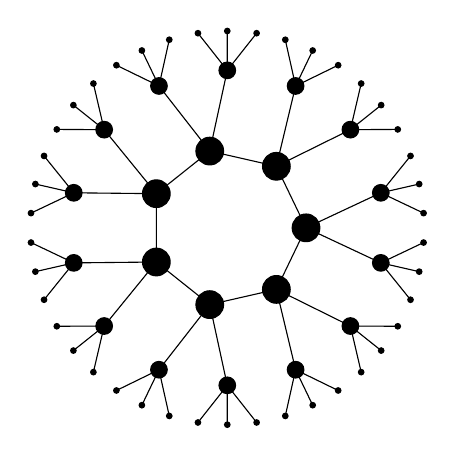
\begin{tikzpicture}[]
      \begin{scope}
        \def\crater{7}
        \foreach \i in {1,...,\crater} {
          \draw[fill] (360/\crater*\i:1cm) circle (5pt);
          \draw (360/\crater*\i : 1cm) -- (360/\crater*\i+360/\crater : 1cm);
          \foreach \j in {-1,1} {
            \draw[fill] (360/\crater*\i : 1cm) -- (360/\crater*\i + \j*360/\crater/4 : 2cm) circle (3pt);
            \foreach \k in {-1,0,1} {
              \draw[fill] (360/\crater*\i + \j*360/\crater/4 : 2cm) --
              (360/\crater*\i + + \j*360/\crater/4 + \k*360/\crater/6 : 2.5cm) circle (1pt);
            }
          }
        }
      \end{scope}
    \end{tikzpicture}
  \end{center}
\end{frame}

%%

\begin{frame}{Endomorphisms}
  \begin{block}{Theorem (Hasse)}
    Let $E$ be defined over a finite field $\F_q$. Its Frobenius map
    $π$ satisfies a quadratic equation
    \[π^2 - tπ + q = 0\] %
    for some \emph{$|t|\le2\sqrt{q}$}, called the \emph{trace}
    of $π$.  The trace $t$ is coprime to $q$ if and only if $E$ is
    ordinary.
  \end{block}
  
  \begin{block}{Endomorphisms}
    An isogeny $E→E$ is also called an \emph{endomorphism}. Examples:
    \begin{itemize}
    \item scalar multiplication \emph{$[n]$},
    \item Frobenius map \emph{$π$}.
    \end{itemize}
    With \emph{addition} and \emph{composition}, the endomorphisms
    form a ring \emph{$\End(E)$}.
  \end{block}
\end{frame}

%%

\begin{frame}{The endomorphism ring}

  \begin{block}{Theorem (Deuring)}
    Let $E$ be an \emph{ordinary} elliptic curve defined over a finite
    field $\F_q$.\\
    Let $π$ be its Frobenius endomorphism, and $D_π=t^2-4q<0$ the
    \emph{discriminant} of its minimal polynomial.

    Then $\End(E)$ is isomorphic to an \emph{order} $\O$ of the
    \emph{quadratic imaginary field} $ℚ(\sqrt{D_π})$.%
    \footnote{An order is a subring that is a $ℤ$-module of rank $2$
      (equiv., a $2$-dimensional $ℝ$-lattice).}
  \end{block}

  In this case, we say that $E$ has \emph{complex multiplication} (CM)
  by $\O$.

  \begin{block}{Theorem (Serre-Tate)}
    CM elliptic curves $E,E'$ are isogenous iff
    \emph{$\End(E)⊗ℚ≃\End(E')⊗ℚ$}.

    \medskip
    
    \textbf{\emph{Corollary:}} $E/\F_p$ and $E'/\F_p$ are isogenous
    over $\F_p$ iff \emph{$\#E(\F_p)=\#E'(\F_p)$}.
  \end{block}

\end{frame}

%%

\begin{frame}{Endomorphism rings of ordinary curves}
  \begin{block}{Classifying quadratic orders}
    Let $K$ be a quadratic number field, and let $\O_K$ be its ring of
    integers.
    \begin{itemize}
    \item Any order $\O\subset K$ can be written as $\O=\Z+f\O_K$ for
      an integer $f$, called the \emph{conductor} of $\O$, denoted by
      $[\O_K:\O]$.
    \item If $D_K$ is the \emph{discriminant} of $K$, the discriminant
      of $\O$ is $f^2D_K$.
    \item If $\O,\O'$ are two orders with discriminants $D,D'$, then
      \emph{$\O\subset\O'$ iff $D'|D$}.
    \end{itemize}
  \end{block}

  \medskip
  
  \centering
  \begin{tikzpicture}[xscale=3,yscale=1.1]
    \node(OK) at (0,0) {$\O_K$};
    \node(O2) at (-1,-1) {$\Z+2\O_K$};
    \node(O3) at (0,-1) {$\Z+3\O_K$};
    \node(O5) at (1,-1) {$\Z+5\O_K$};
    \node(O6) at (-1,-2) {$\Z+6\O_K$};
    \node(O10) at (0,-2) {$\Z+10\O_K$};
    \node(O15) at (1,-2) {$\Z+15\O_K$};
    \node(O30) at (0,-3) {$\Z[\pi]\simeq\Z+30\O_K$};

    \begin{scope}
      \draw
      (OK) edge (O2) edge (O3) edge (O5)
      (O2) edge (O6) edge (O10)
      (O3) edge (O6) edge (O15)
      (O5) edge (O10) edge (O15)
      (O30) edge (O6) edge (O15) edge (O10);
    \end{scope}
  \end{tikzpicture}
\end{frame}

%%%%%%%%%%%%%%%%%%%%%%%%%%%%%%%%%%%%%%%
%%%%%%%%%%%%%%%%%%%%%%%%%%%%%%%%%%%%%%%

\subsection{Ordinary graphs}

\begin{frame}{Volcanology \parencite{kohel}}

  \begin{columns}
    \begin{column}{0.5\textwidth}
      Let \emph{$E,E'$} be curves with respective endomorphism rings \emph{$\O,\O'⊂K$}.\\
      Let \emph{$ϕ:E→E'$} be an isogeny of prime degree \emph{$ℓ$},
      then:
    \end{column}
    \begin{column}{0.5\textwidth}
      \centering{}
      \begin{tabular}{l l}
        if $\O=\O'$, & $ϕ$ is \emph{horizontal};\\
        if $[\O':\O]=ℓ$, & $ϕ$ is \emph{ascending};\\
        if $[\O:\O']=ℓ$, & $ϕ$ is \emph{descending}.
      \end{tabular}      
    \end{column}
  \end{columns}

  \bigskip

  \centering
  \begin{tikzpicture}
    \def\crater{7}
    \foreach \i in {1,...,\crater} {
      \draw[fill] (360/\crater*\i:1cm) circle (5pt);
      \draw (360/\crater*\i : 1cm) -- (360/\crater*\i+360/\crater : 1cm);
      \foreach \j in {-1,1} {
        \draw[fill] (360/\crater*\i : 1cm) -- (360/\crater*\i + \j*360/\crater/4 : 2cm) circle (3pt);
        \foreach \k in {-1,0,1} {
          \draw[fill] (360/\crater*\i + \j*360/\crater/4 : 2cm) --
          (360/\crater*\i + + \j*360/\crater/4 + \k*360/\crater/6 : 2.5cm) circle (1pt);
        }
      }
    }
    \begin{scope}[xshift=4cm]
      \node at (0,2) {$\End(E)$};
      \draw[fill] (0,1) circle(5pt) node[xshift=0.7cm]{$\O_K$} -- 
      (0,0) circle(3pt) --
      (0,-1) circle(1pt) node[xshift=0.7cm]{$ℤ[π]$};
    \end{scope}
  \end{tikzpicture}
  
  \small
  Ordinary isogeny volcano of degree $ℓ=3$.
\end{frame}

%%

\begin{frame}{Volcanology \parencite{kohel}}
  \centering
  \begin{columns}
    \begin{column}{0.35\textwidth}
      Let $E$ be ordinary, \emph{$\End(E)⊂K$}.

      \bigskip

      $\O_K$: \emph{maximal order} of $K$,\\
      $D_K$: \emph{discriminant} of $K$.

      \bigskip
      
      \uncover<2->{Height \emph{$= v_ℓ([\O_K:ℤ[π]])$}.}
      
      \bigskip
      
      \uncover<3->{\alert{How large is the crater?}}
    \end{column}
    \begin{column}{0.65\textwidth}
      \centering
      \begin{tikzpicture}[scale=0.8]
        \small
        \begin{scope}
          \draw[fill] (0,0) circle (2pt)
          -- (-1,-1) circle (2pt)
          (0,0) -- (0,-1) circle (2pt)
          (0,0) -- (1,-1) circle (2pt);
          \node at (0,-2) {$\left(\frac{D_K}{ℓ}\right) = -1$};
        \end{scope}    

        \begin{scope}[xshift=3.5cm]
          \draw[fill] (0,0) circle (2pt)
          -- (-0.5,-1) circle (2pt)
          (0,0) -- (0.5,-1) circle (2pt)
          (0,0) -- (2,0) circle (2pt)
          -- (1.5,-1) circle (2pt)
          (2,0) -- (2.5,-1) circle (2pt);
          \node at (1,-2) {$\left(\frac{D_K}{ℓ}\right) = 0$};
        \end{scope}
        
        \begin{scope}[xshift=2.5cm,yshift=-3cm]
          \draw[fill] (-0.8,0) node[coordinate] (A) {} circle (2pt)
          -- +(0,-1) circle (2pt)
          (0,-0.3) node[coordinate] (B) {} circle (2pt)
          -- +(0,-1) circle (2pt)
          (0.8,0) node[coordinate] (C) {} circle (2pt)
          -- +(0,-1) circle (2pt);
          \draw[bend right=20]
          (A) edge (B)
          (B) edge (C)
          (C) edge[dashed,bend right=90] (A);
          \node at (0,-2) {$\left(\frac{D_K}{ℓ}\right) = +1$};
        \end{scope}
      \end{tikzpicture}
    \end{column}  
  \end{columns}
  
  \bigskip
  
  \begin{tabular}{c | c | c c c}
    && \textbf{Horizontal} & \textbf{Ascending} & \textbf{Descending}\\
    \hline
    $\ell\nmid[\O_K:\O]]$ & $\ell\nmid[\O:ℤ[π]]$ &$1+\left(\frac{D_K}{ℓ}\right)$& &\\
    $\ell\nmid[\O_K:\O]]$ & $\ell\mid[\O:ℤ[π]]$ &$1+\left(\frac{D_K}{ℓ}\right)$& &$\ell-\left(\frac{D_K}{ℓ}\right)$\\
    $\ell\mid[\O_K:\O]]$ & $\ell\mid[\O:ℤ[π]]$ &  &$1$&$\ell$\\
    $\ell\mid[\O_K:\O]]$ & $\ell\nmid[\O:ℤ[π]]$ & &$1$& 
  \end{tabular}
\end{frame}

%%

\begin{frame}{How large is the crater of a volcano?}
  
  Let \emph{$\End(E) = \O \subset ℚ(\sqrt{-D})$}. Define

  \begin{itemize}
  \item $\mathcal{I}(\O)$, the group of \emph{invertible fractional ideals},
  \item $\mathcal{P}(\O)$, the group of \emph{principal ideals},
  \end{itemize}
  
  \begin{block}{The class group}
    The \emph{class group} of $\O$ is
    \[\Cl(\O) = \mathcal{I}(\O)/\mathcal{P}(O).\]
  \end{block}

  \begin{itemize}
  \item It is a \emph{finite abelian} group.
  \item Its order \emph{$h(\O)$} is called the \emph{class number} of
    $\O$.
  \item It arises as the Galois group of an abelian extension of
    $ℚ(\sqrt{-D})$.
  \end{itemize}
\end{frame}

%%

\begin{frame}
  \frametitle{Complex multiplication}
  
  \begin{block}{The $\a$-torsion}
    \begin{itemize}
    \item Let \emph{$\a\subset\O$} be an (integral invertible) ideal of
      $\O$;
    \item Let \emph{$E[\a]$} be the subgroup of $E$ annihilated by
      $\a$:
      \vspace{-2mm}
      \[E[\a] = \{P\in E \;|\; \alpha(P) = 0 \text{ for all } \alpha\in\a\};\]
    \item \vspace{-1mm} Let \emph{$\phi:E\to E_\a$}, where
      $E_\a=E/E[\a]$.
    \end{itemize}
    Then $\End(E_\a) = \O$ (i.e., $\phi$ is \emph{horizontal}).
  \end{block}


  \begin{theorem}[Complex multiplication]
    The action on the set of elliptic curves with complex
    multiplication by $\O$ defined by \emph{$\a\ast j(E) = j(E_\a)$}
    factors through $\Cl(\O)$, is faithful and transitive.
  \end{theorem}

  \begin{corollary}
    Let $\End(E)$ have discriminant $D$. Assume that
    $\left(\frac{D}{\ell}\right)=1$, then $E$ is on a crater \emph{of
      size $N$} of an $\ell$-volcano, and \emph{$N|h(\End(E))$}
  \end{corollary}
\end{frame}

%%

\begin{frame}
  \frametitle{Complex multiplication graphs}
  \begin{center}
    \begin{tikzpicture}
      \begin{scope}
        \def\crater{12}
        \def\jumpa{-8}
        \def\jumpb{9}
        \def\diam{3cm}

        \foreach \i in {1,...,\crater} {
          \uncover<2->{\draw[blue] (360/\crater*\i : \diam) to[bend right] (360/\crater*\i+360/\crater : \diam);}
          \uncover<3->{\draw[red] (360/\crater*\i : \diam) to[bend right] (360/\crater*\i+\jumpa*360/\crater : \diam);}
          \uncover<4->{\draw[green] (360/\crater*\i : \diam) to[bend right=50] (360/\crater*\i+\jumpb*360/\crater : \diam);}
        }
        \foreach \i in {1,...,\crater} {
          \draw[fill] (360/\crater*\i: \diam) circle (2pt) +(360/\crater*\i: 0.4) node{$E_{\i}$};
        }
      \end{scope}
      \begin{scope}[xshift=4cm]
        \draw (0,2.5) node[anchor=west] {\parbox{4cm}{%
            Vertices are elliptic curves \emph{with complex
              multiplication by $\O_K$} (i.e., $\End(E)\simeq\O_K\subset ℚ(\sqrt{-D})$).\\
            \uncover<2->{Edges are \emph{horizontal isogenies} of
              bounded prime degree.}  }};
      
        \uncover<2->{\draw[blue] (0,0) -- (0.5,0)
          (0.5,0) node[anchor=west] {degree $2$};}
        \uncover<3->{\draw[red] (0,-1) -- (0.5,-1) (0.5,-1)
          node[anchor=west] {degree $3$};}
        \uncover<4->{\draw[green]
          (0,-2) -- (0.5,-2) (0.5,-2) node[anchor=west] {degree $5$};}

        \uncover<5->{\draw (0,-3) node[anchor=west] {\parbox{4cm}{%
              Isomorphic to a \emph{Cayley graph of $\Cl(\O_K)$}.}};}
      \end{scope}
    \end{tikzpicture}
  \end{center}
\end{frame}

%% 

{
  \newcommand{\myedge}[3]{
    \draw[#3] (360/\crater*#1 : \diam) to[bend right] (360/\crater*#2 : \diam);
  }

\begin{frame}
  \frametitle{\alt<7->{Couveignes--Rostovtsev--Stolbunov key exchange}{Key exchange from Cayley graphs}}

  \begin{columns}
    \begin{column}{0.55\textwidth}
      \begin{tikzpicture}
        \begin{scope}
          \def\crater{12}
          \def\jumpa{-8}
          \def\jumpb{9}
          \def\diam{2.5cm}
          
          \foreach \i in {1,...,\crater} {
            \pgfmathparse{int(mod(2^\i,13))}
            \let\exp\pgfmathresult
            \draw[fill] (360/\crater*\i: \diam) circle (2pt);
          }
          \uncover<2,6->{
            % Alice 1
            \myedge{0}{1}{blue}\myedge{1}{5}{red}\myedge{5}{6}{blue}\myedge{6}{3}{green}
          }
          \uncover<3,5>{
            % Bob 1
            \begin{scope}[dashed,thick]
              \myedge{0}{4}{red}\myedge{4}{8}{red}\myedge{8}{5}{green}\myedge{5}{6}{blue}
            \end{scope}
          }
          \uncover<5>{
            % Alice 2
            \myedge{6}{7}{blue}\myedge{7}{11}{red}\myedge{11}{0}{blue}\myedge{0}{9}{green}
          }
          \uncover<6->{
            % Bob 2
            \begin{scope}[dashed,thick]
              \myedge{3}{7}{red}\myedge{7}{11}{red}\myedge{11}{8}{green}\myedge{8}{9}{blue}
            \end{scope}
          }

          \draw (0 : \diam + 0.4cm) node {\alt<7->{$E$}{$x$}};
          \uncover<2->{\draw (360/\crater*3 : \diam + 0.4cm) node {\alt<7->{$E_A$}{$x_A$}};}
          \uncover<3->{\draw (360/\crater*6 : \diam + 0.4cm) node {\alt<7->{$E_B$}{$x_B$}};}
          \uncover<5->{\draw (360/\crater*9 : \diam + 0.4cm) node {\alt<7->{$E_{B}=E_{AB}$}{$x_{BA}\uncover<6->{=x_{AB}}$}};}
        \end{scope}
      \end{tikzpicture}  
    \end{column}    
    \begin{column}{0.45\textwidth}
      \begin{onlyenv}<-6>
        \textbf{Public parameters:}
        \begin{itemize}
        \item A commutative group \emph{$G$} acting on a set \emph{$X$};
        \item A starting point \emph{$x\in X$};
        \item A subset
          \emph{$G\supset S=\{\bl{s_1},\rd{s_2},\gr{s_3},\dots\}$}.
        \end{itemize}
        \begin{enumerate}
        \item<2-> \textbf{Alice} takes a secret random walk
          \emph{$s_A=\bl{s_1^{e_1}}\cdot\rd{s_2^{e_2}}\cdot\gr{s_3^{e_3}}\cdots$}
          landing on \emph{$x_A=s_A*x$};
        \item<3-> \textbf{Bob} does the same;
        \item<4-> They publish \emph{$x_A$} and \emph{$x_B$};
        \item<5-> \textbf{Alice} repeats her secret walk \emph{$s_A$}
          starting from \emph{$x_B$}.
        \item<6-> \textbf{Bob} repeats his secret walk \emph{$s_B$}
          starting from \emph{$x_A$}.
        \end{enumerate}
      \end{onlyenv}
      \begin{onlyenv}<7->
        \textbf{Now, with isogenies}
        \begin{itemize}
        \item \emph{$G=\Cl(\O_K)$}, a class group;
        \item \emph{$X=$} elliptic curves with CM by \emph{$\O_K$};
        \item A starting curve \emph{$E$};
        \item \emph{$S=$} set of small degree isogenies.
        \end{itemize}
        \uncover<8->{\textbf{But why?!}}

        \uncover<9->{Because the Shor/Kitaev \emph{quantum} algorithm
          \emph{does not apply} to Diffie-Hellman on Cayley graphs!}
      \end{onlyenv}
    \end{column}
  \end{columns}
\end{frame}
}

%% 

\begin{frame}{CSIDH {\small (pron.: \textit{sea-side})}}
  \begin{block}{Speeding up the CRS key
      exchange \parencite{10.1007/978-3-030-03332-3_14}}
    \begin{itemize}
    \item Choose \emph{$p$} such that \emph{$\ell\mid(p+1)$} for many
      small primes \emph{$\ell$};
    \item Look for random \emph{ordinary} curves such that: \hfill\alert{HARD!}
      \begin{itemize}
      \item \emph{$\ell\mid E(\F_p)$},
      \item technical condition;
      \end{itemize}
    \item Use Vélu's formulas for \emph{those primes $\ell$}.
    \item $\sim$5 minutes for a 128-bit secure key exchange \hfill\alert{\Sadey}
    \end{itemize}
  \end{block}

  \begin{block}{CSIDH \parencite{10.1007/978-3-030-03332-3_15}}
    \begin{itemize}
    \item Choose \emph{$p$} such that \emph{$\ell\mid(p+1)$} for many
      small primes \emph{$\ell$};
    \item Select a \emph{supersingular} curve \emph{$E/\F_p$},
      automatically \hfill\alert{EASY!}
      \begin{itemize}
      \item \emph{$\#E(\F_p)=p+1$},
      \item technical condition always satisfied;
      \end{itemize}
    \item $\sim$100ms for a 128 bits secure key exchange \hfill\alert{\Smiley}
    \end{itemize}
  \end{block}
\end{frame}

%%

\begin{frame}{Supersingular graphs}
  \begin{columns}
    \begin{column}{0.6\textwidth}
      \begin{itemize}
      \item Quaternion algebras have \emph{many maximal orders}.
      \item For every \emph{maximal order type} of $B_{p,\infty}$
        there are \emph{$1$ or $2$ curves over $\F_{p^2}$} having
        endomorphism ring isomorphic to it.
      \item There is a \emph{unique isogeny class} of supersingular
        curves over $\bar{\F}_p$ of size \emph{$≈ p/12$}.
      \item Left ideals act on the set of maximal orders like isogenies.
      \item The graph of \emph{$\ell$}-isogenies is
        \emph{$(\ell+1)$}-regular.
      \end{itemize}
    \end{column}
    \begin{column}{0.4\textwidth}
      \centering
      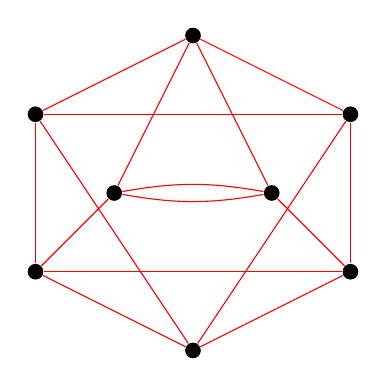
\begin{tikzpicture}
        \begin{scope}[every node/.style={fill,black,circle,inner sep=2pt}]
          \node at (0,0)  (1){};
          \node at (0,4) (20){};
          \node at (2,1)  (16z){};
          \node at (-2,1)  (81z){};
          \node at (-1,2) (77z){};
          \node at (1,2)  (20z){};
          \node at (-2,3)  (85z){};
          \node at (2,3)  (12z){};
        \end{scope}

        \begin{scope}[red]
          \path (1) edge (85z) edge (81z) edge (12z) edge (16z);
          \path (20) edge (85z) edge (77z) edge (20z) edge (12z);
          \path (81z) edge (85z) edge (77z) edge (16z);
          \path (85z) edge (12z);
          \path (12z) edge (16z);
          \path (16z) edge (20z);
          \path (20z) edge[bend right=10] (77z) edge[bend left=10] (77z);
        \end{scope}
      \end{tikzpicture}
      \small
      \emph{Figure:} $3$-isogeny graph on $\F_{97^2}$.
    \end{column}
  \end{columns}
\end{frame}

%%

\begin{frame}
  \frametitle{Key exchange with full supersingular graphs (over $\F_{p^2}$)}
  
  \begin{description}
  \item[Good news:] there is no action of a commutative class group.
  \item[Bad news:] there is no action of a commutative class group.
  \item[Idea:] Let \bl{Alice} and \rd{Bob} walk in two
    \emph{different isogeny graphs} on the \emph{same vertex set}.
  \end{description}

  \begin{columns}
    \begin{column}{0.7\textwidth}
      \centering
      \begin{tikzpicture}[scale=1.4]
        \begin{scope}[every node/.style={fill,black,circle,inner sep=2pt}]
          \node at (0,0)  (1){};
          \node at (0,4) (20){};
          \node at (2,1)  (16z){};
          \node at (-2,1)  (81z){};
          \node at (-1,2) (77z){};
          \node at (1,2)  (20z){};
          \node at (-2,3)  (85z){};
          \node at (2,3)  (12z){};
        \end{scope}

        \begin{uncoverenv}<1,3>
          \begin{scope}[blue,every loop/.style={looseness=50}]
            \path (1) edge (20) edge (16z) edge (81z);
            \path (20) edge[loop left] (20) edge[loop right] (20);
            \path (16z) edge (81z) edge (77z);
            \path (81z) edge (20z);
            \path (77z) edge (20z) edge (85z);
            \path (20z) edge (12z);
            \path (12z) edge[bend right=10] (85z) edge[bend left=10] (85z);
          \end{scope}
        \end{uncoverenv}
        
        \begin{uncoverenv}<2->
          \begin{scope}[red]
            \path (1) edge (85z) edge (81z) edge (12z) edge (16z);
            \path (20) edge (85z) edge (77z) edge (20z) edge (12z);
            \path (81z) edge (85z) edge (77z) edge (16z);
            \path (85z) edge (12z);
            \path (12z) edge (16z);
            \path (16z) edge (20z);
            \path (20z) edge[bend right=10] (77z) edge[bend left=10] (77z);
          \end{scope}
        \end{uncoverenv}
      \end{tikzpicture}
    \end{column}
    \begin{column}{0.3\textwidth}
      \small
      \emph{Figure:} \bl{$2$}- and \rd{$3$}-isogeny graphs on $\F_{97^2}$.
    \end{column}
  \end{columns}
\end{frame}

%%

\begin{frame}
  \frametitle{Key exchange with full supersingular graphs (over $\F_{p^2}$)}

  \begin{itemize}
  \item Fix small primes \bl{$\ell_A$}, \rd{$\ell_B$};
  \item \emph{No canonical labeling} of the \bl{$\ell_A$}- and
    \rd{$\ell_B$}-isogeny graphs; \emph{however\dots}
  \end{itemize}

  \begin{center}
    \bf
    Walk of length \bl{$e_A$}\\
    $=$\\
    Isogeny of degree \bl{$\ell_A^{e_A}$}\\
    $=$\\
    Kernel \bl{$\langle P\rangle\subset E[\ell_A^{e_A}]$}
  \end{center}
  
  \begin{center}
    \begin{tikzpicture}
      \begin{scope}
        \draw (0,1.2) node[anchor=east,blue] {$\ker\phi=\cyc{P}\subset E[\ell_A^{e_A}]$};
        \draw (0,0.4) node[anchor=east,red] {$\ker\psi=\cyc{Q}\subset E[\ell_B^{e_B}]$};
        \draw (0,-0.4) node[anchor=east,blue] {$\ker\phi' = \cyc{\rd{\psi}(P)}$};
        \draw (0,-1.2) node[anchor=east,red] {$\ker\psi' = \cyc{\bl{\phi}(Q)}$};
      \end{scope}
      \begin{scope}[xshift=4.5cm,coils/.style={-angle 90,decorate,decoration={coil,aspect=0,amplitude=1pt}}]
        \large
        \node[matrix of nodes, ampersand replacement=\&, column sep=3cm, row sep=1.5cm] (diagram) {
          |(E)| $E$ \& |(Es)| $E/\cyc{\bl{P}}$ \\
          |(Ep)| {$E/\cyc{\rd{Q}}$} \& |(Eps)| {$E/\cyc{\bl{P},\rd{Q}}$}\\
        };
        \path[->,blue] (E) edge[coils] node[auto] {$\phi$} (Es);
        \path[->,blue] (Ep) edge[coils] node[auto,swap] {$\phi'$} (Eps);
        \path[->,red] (E) edge[coils] node[auto,swap] {$\psi$} (Ep);
        \path[->,red] (Es) edge[coils] node[auto] {$\psi'$} (Eps);
      \end{scope}
    \end{tikzpicture}
  \end{center}
\end{frame}

%%

\begin{frame}{SIKE: Supersingular Isogeny Key Encapsulation}
  \begin{itemize}
  \item Submission to the \emph{NIST PQ competition}:
    \begin{description}
    \item[SIKE.PKE:] El Gamal-type system with \emph{IND-CPA} security
      proof,
    \item[SIKE.KEM:] generically transformed system with
      \emph{IND-CCA} security proof.
    \end{description}
  \item Security levels 1, 3 and 5.
  \item \emph{Smallest communication complexity} among all proposals
    in each level.
  \item \emph{Slowest} among all benchmarked proposals in each level.
  \item A team of 14 submitters, from 8 universities and companies.
  \item Visit \emph{\href{https://sike.org/}{https://sike.org/}}.
  \end{itemize}

  \centering
  \begin{tabular}{l | c c c c c }
    & $p$ & cl. security & q. security & speed & comm.\\
    \hline
    SIKEp503 & $2^{250}3^{159}-1$ & 126 bits & 84 bits & 10ms & 0.4KB\\
    SIKEp751 & $2^{372}3^{239}-1$ & 188 bits & 125 bits & 30ms & 0.6KB\\
    SIKEp964 & $2^{486}3^{301}-1$ & 241 bits & 161 bits & & 0.8KB
  \end{tabular}
\end{frame}

%%

\begin{frame}{From 10 minutes to 10ms in 20 years}
  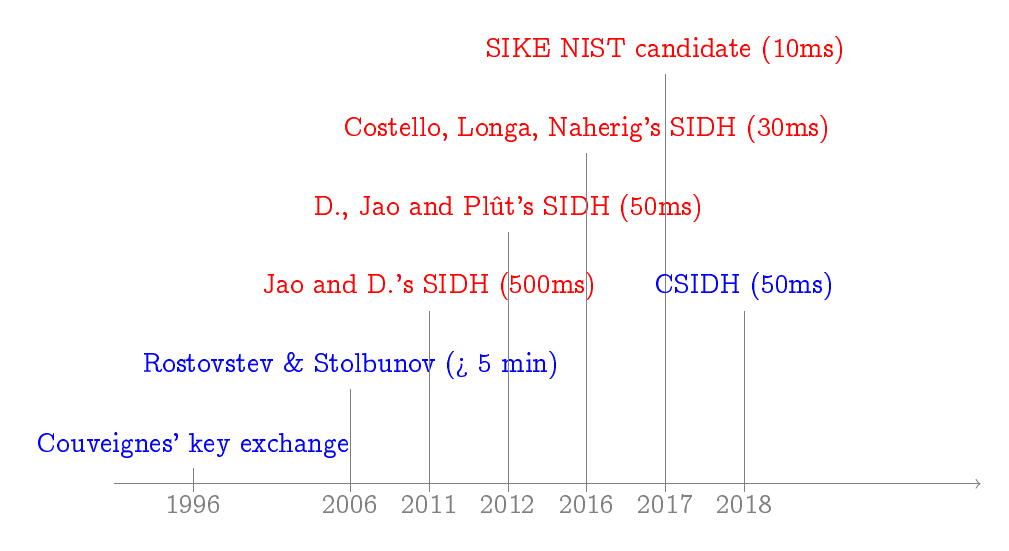
\begin{tikzpicture}[gray,every node/.style={anchor=south}]
    \draw[->] (0,0) -- (11,0);
    \uncover<1->{
      \node at (1,-0.5) {1996};
      \draw (1,-0.1) -- +(0,0.3) node[blue]{Couveignes' key exchange};
    }
    \uncover<2->{
      \node at (3,-0.5) {2006};
      \draw (3,-0.1) -- +(0,1.3) node[blue]{Rostovstev \& Stolbunov (> 5 min)};
    }
    \uncover<3->{
      \node at (4,-0.5) {2011};
      \draw (4,-0.1) -- +(0,2.3) node[red]{Jao and D.'s SIDH (500ms)};
    }
    \uncover<4->{
      \node at (5,-0.5) {2012};
      \draw (5,-0.1) -- +(0,3.3) node[red]{D., Jao and Plût's SIDH (50ms)};
    }
    \uncover<5->{
      \node at (6,-0.5) {2016};
      \draw (6,-0.1) -- +(0,4.3) node[red]{Costello, Longa, Naherig's SIDH (30ms)};
    }
    \uncover<6->{
      \node at (7,-0.5) {2017};
      \draw (7,-0.1) -- +(0,5.3) node[red]{SIKE NIST candidate (10ms)};
    }
    \uncover<7->{
      \node at (8,-0.5) {2018};
      \draw (8,-0.1) -- +(0,2.3) node[blue]{CSIDH (50ms)};
    }
  \end{tikzpicture}
\end{frame}

%%

\begin{frame}{Open problems}
  From easier to harder:
  \begin{itemize}
  \item Give a convincing constant-time implementation of CSIDH.
  \item Find new isogeny-based primitives/protocols.
  \item Precisely asses the quantum security of CRS/CSIDH.
  \item Find an efficient post-quantum isogeny-based signature scheme.
  \item Exploit the extra information transmitted in SIDH/SIKE for
    cryptanalytic purposes.
  \item Sample supersingular curves without revealing endomorphism
    rings.
  \item Compute endomorphism rings of supersingular curves.
  \end{itemize}
\end{frame}

%%

%%

\begin{frame}
  \centering
  \begin{tikzpicture}
    \begin{scope}[xscale=1.2,black!60]
      \def\crater{7}
      \foreach \i in {1,...,\crater} {
        \draw[fill] (360/\crater*\i:3cm) circle (5pt);
        \draw (360/\crater*\i : 3cm) -- (360/\crater*\i+360/\crater : 3cm);
        \foreach \j in {-1,1} {
          \draw[fill] (360/\crater*\i : 3cm) -- (360/\crater*\i + \j*360/\crater/4 : 4cm) circle (3pt);
          \foreach \k in {-1,0,1} {
            \draw[fill] (360/\crater*\i + \j*360/\crater/4 : 4cm) --
            (360/\crater*\i + + \j*360/\crater/4 + \k*360/\crater/6 : 4.5cm) circle (1pt);
          }
        }
      }
    \end{scope}
    
    \draw (0,1) node{\Huge\bf Thank you};
    \draw (0,-0.6) node{\large\url{https://defeo.lu/}};
    \draw (0,-1.3) node{\large
\includegraphics[height=0.9em]{twitter.png}~\href{https://twitter.com/luca_defeo}{@luca\_defeo}};
  \end{tikzpicture}
\end{frame}

%%

\begin{frame}{CSIDH vs SIDH}
  \centering
  \vspace{-3mm}
  \begin{tabular}{l | c | c}
    & \textbf{CSIDH} & \textbf{SIDH}\\
    \hline
    Speed (NIST 1) & <100ms & $\sim$ 10ms\\
    Public key size (NIST 1) & 64B & 378B\\
    Key compression\footcite{10.1007/978-3-319-79063-3_12} & \\
    \enskip{}\rotatebox[origin=c]{180}{$\Lsh$} speed & & $\sim$ 15ms\footnote{https://twitter.com/PatrickLonga/status/1002313366466015232?s=20}\\
    \enskip{}\rotatebox[origin=c]{180}{$\Lsh$} size & & 222B\\
    Constant time impl. & not yet & yes\\
    Submitted to NIST & no & yes\\
    \hline
    Best classical attack & $p^{1/4}$ & $p^{1/4}$\\
    Best quantum attack & $\tildO\left(3^{\sqrt{\log_3 p}}\right)$ & $p^{1/6}$\\
    Key size scales & quadratically & linearly\\
    Security assumption & isogeny walk problem & ad hoc\\
    CPA security & yes & yes\\
    CCA security & yes & Fujisaki-Okamoto\\
    \hline
    Non-interactive key ex. & yes & no\\
    Signatures & short but slooow! & big and slow
  \end{tabular}
\end{frame}

%%

\begin{frame}{Signatures {\small (a different story)}}
  \begin{itemize}
  \item No analogue of \emph{Schnorr signatures} for DH on Cayley
    graphs.
  \item All known isogeny constructions are basic \emph{Fiat-Shamir}
    applied to zero-knowledge identification protocols.
  \end{itemize}

  \begin{block}{SIDH signatures}
    \begin{itemize}
    \item Identification protocol also proposed by D.F., Jao, Plût;
    \item Only \emph{one bit per iteration} $\to$ 128 iterations
      of SIDH primitive;
    \item Slow, large signatures;
    \item Even slower variants by \cite{cryptoeprint:2016:1154}.
    \end{itemize}
  \end{block}

  \begin{block}{CSIDH signatures (SeaSign)}
    \begin{itemize}
    \item (Flawed) id protocol already realized by
      Couveignes, Stolbunov;
    \item SeaSign \parencite{SeaSign}: fixes flaw using
      \emph{Fiat-Shamir with aborts} \parencite{Lyu09} \emph{\small(+
        hash trees)};
    \item Small signatures, still extremely slow (minutes).
    \end{itemize}
  \end{block}
\end{frame}

\begin{frame}[allowframebreaks]
  \frametitle{Article citations}

  \defbibfilter{books}{\type{book} \or \type{booklet} \or \type{thesis}
    \or \type{report} \or \type{collection} \or \type{manual}
    \or \type{periodical} \or \type{proceedings}}
  \defbibfilter{articles}{\not \(\type{book} \or \type{booklet} \or \type{thesis}
    \or \type{report} \or \type{collection} \or \type{manual}
    \or \type{periodical} \or \type{proceedings}\)}

%  \beamertemplatebookbibitems
%  \printbibliography[filter=books]
  \beamertemplatearticlebibitems
  \printbibliography[filter=articles]
\end{frame}

\end{document}


% LocalWords:  Isogeny abelian isogenies hyperelliptic supersingular Frobenius
% LocalWords:  isogenous


